\chapter{基于FAST\_LIO2的激光里程计定位算法研究}
\section{实时定位与地图构建（SLAM）}
实时定位与地图构建（Simultaneous Localization and Mapping）是移动机器人与自动驾驶领域的核心技术。其核心任务可归结为一种耦合估计问题：
在未知环境中，移动平台利用传感器数据，同步完成对自身运动状态的描述与对环境空间结构的建模。二者相互依赖，定位精度依赖于地图的准确性，
而一致地图的构建又需以精确的位姿轨迹为前提。
\section{SLAM方法架构及技术分类}
实时定位与地图构建作为一个复杂的状态估计问题，其解决方案已形成相对统一的系统架构。一个完整的SLAM系统通常包含以下几个关键模块：
前端里程计、后端优化、建图模块以及回环检测模块。传感器层面可分为激光雷达SLAM、视觉SLAM及多传感器融合SLAM，后端框架层面可分为基于滤波器的SLAM和基于图优化的SLAM。

前端里程计负责对相邻时刻的传感器数据进行关联与配准，实时估计传感器平台的增量运动，形成局部一致的轨迹与地图，
但其误差会随时间累积。后端优化则接收前端输出的位姿估计以及回环检测模块提供的非连续时刻的约束信息，构建一个以位姿为节点、以约束为边的概率图模型，
并通过非线性优化方法求解全局一致的最优轨迹。建图模块利用优化后的轨迹，将传感器观测数据融合到统一坐标系下，生成环境地图。
根据核心框架与传感器类型的不同，SLAM技术可进行如下分类：从传感器层面，主要分为激光雷达SLAM、视觉SLAM以及多传感器融合SLAM；
从后端框架层面，则主要分为基于滤波器的SLAM与基于图优化的SLAM两大类。

\subsection{基于滤波器的SLAM}
基于滤波器的SLAM方法将系统的状态（包括机器人位姿与环境路标点）建模为一个随时间演进的概率分布。
其核心思想是采用递归的贝叶斯估计框架，在每一时刻，根据当前的控制输入和传感器观测，对系统状态的置信度（后验概率）进行更新。
最具代表性的方法是扩展卡尔曼滤波器（EKF-SLAM）及其改进算法。EKF-SLAM通过线性化非线性运动与观测模型，在状态向量的高斯分布假设下，进行均值和协方差的递推更新。
此类方法的优势在于能够提供状态的在线估计及其不确定性度量，且计算复杂度与路标数量相关。然而，其线性化误差可能导致滤波器发散，且通常假设数据关联是已知或准确的。
FastSLAM算法通过粒子滤波估计路径，结合EKF估计路标，部分克服了EKF-SLAM的局限性，但粒子退化问题依然存在。在计算资源受限、强调实时性的应用场景中，基于滤波器的轻量化变体（如迭代卡尔曼滤波）仍具有重要价值。

\subsection{基于图优化的SLAM}
基于图优化的SLAM是当前主流的高精度SLAM框架。该方法将SLAM问题转化为一个大规模非线性最小二乘优化问题。其模型是一个图结构：节点表示机器人不同时刻的位姿（有时也包括环境路标），边则表示位姿节点之间的空间约束。
边主要分为两种：一是由前端里程计产生的连续位姿间的约束（里程计边），二是由回环检测产生的非连续位姿间的约束（回环边）。当检测到回环时，相当于在图中添加了新的强约束，
从而能够有效校正累积的里程计漂移。优化目标是寻找一组最优的节点状态（位姿），使得图中所有边代表的预测观测与实际观测之间的误差平方和最小。常用的优化工具包括高斯-牛顿法、列文伯格-马夸尔特算法等。
与滤波器方法相比，图优化方法能更自然地融合回环约束，进行全局一致性优化，从而获得精度更高的轨迹和地图，但其通常作为后端批量或滑动窗口优化运行，对计算资源要求较高。g2o、GTSAM、Ceres Solver等开源库为图优化SLAM的实现提供了强大支撑。

\subsection{紧耦合激光-惯性SLAM}
紧耦合激光-惯性SLAM是当前实现高鲁棒性、高频率状态估计的主流方案，其核心在于对激光雷达与惯性测量单元（IMU）的数据进行深层次融合。IMU能够以数百赫兹的频率测量角速度和加速度，在短时间内积分可提供高频但快速发散的位姿预测。
激光雷达则提供低频但绝对精度较高的三维几何观测。紧耦合方法并非将二者独立处理后再进行结果融合，而是在一个统一的状态估计框架内，直接使用原始的激光雷达点云和IMU测量值，共同约束系统状态（通常包括位置、姿态、速度、传感器偏置等）。
具体而言，激光雷达的每一个或多个原始点都可以直接作为观测方程，与IMU预测的运动方程一起，构建一个状态估计问题。这种深度融合方式充分利用了IMU的高频动态信息来辅助激光雷达点云的运动畸变矫正和数据关联，同时利用激光雷达的精确观测来抑制IMU积分漂移。
以FAST-LIO系列为代表的算法，通过将紧耦合的激光-惯性里程计建模在迭代卡尔曼滤波框架下，实现了在剧烈运动场景中的鲁棒、实时、高精度状态估计，是紧耦合SLAM的典型代表\textsuperscript{\cite{Xu2021FASTLIO}}。

\section{FAST\_LIO2激光惯性里程计原理}
FAST\_LIO2是一类面向实时三维建图与定位的紧耦合激光惯性里程计方法，其核心思想是在误差状态迭代卡尔曼滤波框架内融合IMU传播模型与激光点云到局部地图的几何约束\textsuperscript{\cite{Xu2022FASTLIO2}}。与LOAM类方法先提取边缘点、平面点再进行特征匹配的流程不同\textsuperscript{\cite{Zhang2014LOAM}}，FAST\_LIO2取消了手工特征提取模块，直接使用降采样后的原始激光点与地图进行配准。这种直接法能够保留更多环境几何信息，降低算法对雷达扫描模式和特征阈值的依赖，因此更适合Livox MID360等非重复扫描或小型移动平台常用的三维激光雷达。

FAST\_LIO2的系统流程可概括为：首先，利用IMU高频测量对状态进行前向传播，并在传播过程中对一帧激光点云内部的运动畸变进行补偿；其次，将去畸变后的点云变换到世界坐标系，在增量地图中搜索近邻点并拟合局部平面；最后，根据点到局部平面的残差构造量测模型，通过迭代卡尔曼滤波更新位姿、速度、IMU偏置以及外参等状态。为保证实时性，FAST\_LIO2采用增量式$k$维树（ikd-Tree）维护点云地图，使地图能够在线支持点插入、删除、重平衡和近邻搜索，避免每一帧重新构建静态KD树带来的高计算开销\textsuperscript{\cite{Cai2021ikdTree}}。

\begin{figure}[htbp]
  \centering
  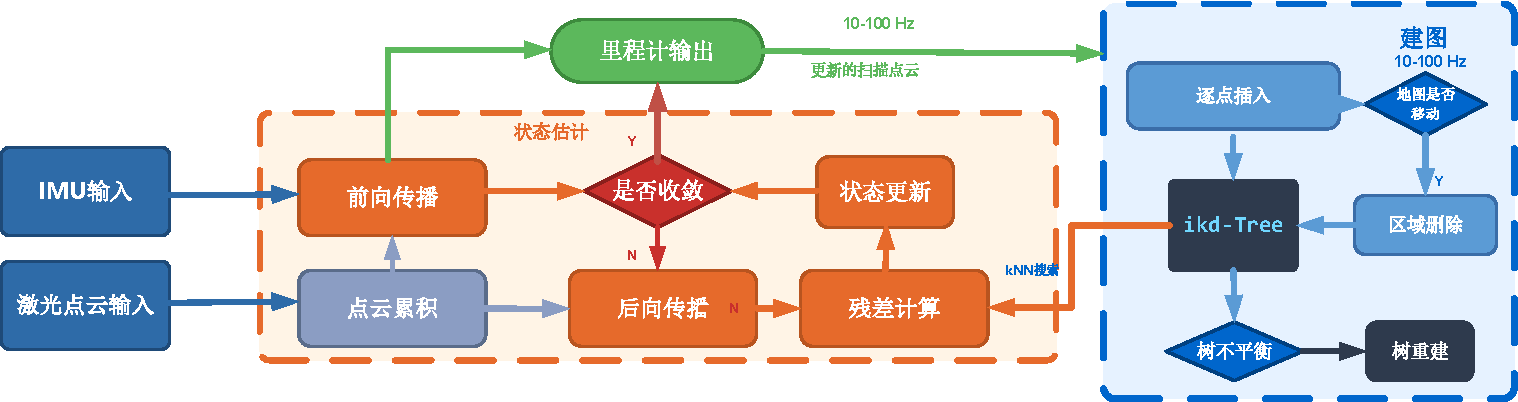
\includegraphics[width=\linewidth]{pic/激光惯性里程计系统架构.pdf}
  \caption{FAST-LIO2激光惯性里程计系统架构}
  \label{fig:fastlio_arch}
\end{figure}

系统由两大模块组成：
    （1）状态估计模块（橙色虚线框）：基于迭代误差状态卡尔曼滤波（IEKF），
    通过IMU前向传播、点云累积、后向传播、残差计算和状态更新的迭代循环，
    输出高频位姿估计；
   （2）建图模块（蓝色虚线框）：基于增量式kd树（ikd-Tree）维护局部点云地图，
    支持逐点插入、树上降采样、区域删除和动态重平衡，
    为状态估计提供kNN近邻搜索服务。
    输出的里程计位姿（绿色）既作为导航反馈，也驱动地图更新和前向传播的初值。

\subsection{状态变量与IMU传播模型}
图\ref{fig:fastlio_arch}展示了FAST\_LIO2的完整系统架构。其核心是状态估计与建图的紧密协同：IMU提供连续高频运动预测，激光雷达提供离散低频几何观测，二者在误差状态迭代卡尔曼滤波框架内深度融合。具体而言，系统在每帧同步数据到来时，首先利用IMU测量进行前向传播并补偿点云运动畸变；随后将去畸变点云累积并变换到世界坐标系，在ikd-Tree维护的增量地图中搜索近邻点，拟合局部平面并计算点到平面残差；最后通过迭代优化更新状态。当残差收敛时，输出当前位姿作为里程计结果并反馈至下一帧的前向传播初值；若未收敛，则继续后向传播进行下一轮迭代。建图模块根据输出位姿判断是否需要地图移动或区域删除，并将新观测点按体素分辨率插入ikd-Tree，保持地图的实时性与紧凑性。

设系统状态定义为
\begin{equation}
    \mathbf{x}
    =
    \left[
    {}^{G}\mathbf{p}_{I}^{T},
    {}^{G}\mathbf{R}_{I},
    {}^{I}\mathbf{R}_{L},
    {}^{I}\mathbf{p}_{L}^{T},
    {}^{G}\mathbf{v}_{I}^{T},
    \mathbf{b}_{g}^{T},
    \mathbf{b}_{a}^{T},
    {}^{G}\mathbf{g}^{T}
    \right],
    \label{eq:fastlio_state}
\end{equation}
其中${}^{G}\mathbf{p}_{I}$、${}^{G}\mathbf{R}_{I}$分别表示IMU坐标系相对于全局坐标系的位置和姿态，${}^{I}\mathbf{R}_{L}$、${}^{I}\mathbf{p}_{L}$表示激光雷达相对于IMU的外参，${}^{G}\mathbf{v}_{I}$为IMU速度，$\mathbf{b}_{g}$、$\mathbf{b}_{a}$分别为陀螺仪和加速度计偏置，${}^{G}\mathbf{g}$为重力向量。上述状态同时包含运动状态、传感器误差项和外参项，使激光几何约束能够与惯性传播约束在同一估计框架内共同作用。

IMU测量可表示为
\begin{equation}
    \boldsymbol{\omega}_{m}=\boldsymbol{\omega}+\mathbf{b}_{g}+\mathbf{n}_{g},
    \quad
    \mathbf{a}_{m}=\mathbf{a}+\mathbf{b}_{a}+\mathbf{n}_{a},
    \label{eq:imu_measurement}
\end{equation}
其中$\boldsymbol{\omega}_{m}$和$\mathbf{a}_{m}$为IMU输出的角速度和加速度，$\mathbf{n}_{g}$、$\mathbf{n}_{a}$为测量噪声。连续时间状态传播可写为
\begin{equation}
\begin{aligned}
    {}^{G}\dot{\mathbf{p}}_{I} &= {}^{G}\mathbf{v}_{I},\\
    {}^{G}\dot{\mathbf{R}}_{I} &= {}^{G}\mathbf{R}_{I}
    \left(\boldsymbol{\omega}_{m}-\mathbf{b}_{g}-\mathbf{n}_{g}\right)^{\wedge},\\
    {}^{G}\dot{\mathbf{v}}_{I} &= {}^{G}\mathbf{R}_{I}
    \left(\mathbf{a}_{m}-\mathbf{b}_{a}-\mathbf{n}_{a}\right)
    +{}^{G}\mathbf{g},\\
    \dot{\mathbf{b}}_{g} &= \mathbf{n}_{bg},\quad
    \dot{\mathbf{b}}_{a} = \mathbf{n}_{ba}.
\end{aligned}
    \label{eq:imu_propagation}
\end{equation}
式中$(\cdot)^{\wedge}$表示李代数向量到反对称矩阵的映射。由于激光雷达在采集一帧点云时平台仍在连续运动，若直接将整帧点云视为同一时刻采集，会在快速转弯或加减速时产生明显运动畸变。FAST\_LIO2利用IMU传播得到的连续位姿，对每个点按照其相对时间戳进行反向补偿，将其统一到该帧结束时刻，从而提升后续点云配准的一致性。

\subsection{直接点到地图量测模型}
在量测更新阶段，FAST\_LIO2将去畸变后的激光点${}^{L}\mathbf{p}_{j}$根据当前状态变换到全局坐标系：
\begin{equation}
    {}^{G}\mathbf{p}_{j}
    =
    {}^{G}\mathbf{R}_{I}
    \left(
    {}^{I}\mathbf{R}_{L}{}^{L}\mathbf{p}_{j}
    +{}^{I}\mathbf{p}_{L}
    \right)
    +{}^{G}\mathbf{p}_{I}.
    \label{eq:point_transform}
\end{equation}
随后在ikd-Tree维护的地图中搜索该点的若干近邻点，并利用近邻点拟合局部平面
\begin{equation}
    \mathbf{u}_{j}^{T}\mathbf{p}+d_{j}=0,
    \label{eq:local_plane}
\end{equation}
其中$\mathbf{u}_{j}$为平面单位法向量，$d_{j}$为平面参数。对应的点到平面残差为
\begin{equation}
    r_{j}
    =
    \mathbf{u}_{j}^{T}{}^{G}\mathbf{p}_{j}
    +d_{j}.
    \label{eq:point_plane_residual}
\end{equation}
该残差直接反映当前状态估计下激光点与局部地图几何的一致性。实际量测构造过程包括坐标变换、近邻搜索、局部平面估计、残差筛选和量测雅可比计算等步骤。当有效点数量不足或近邻无法稳定拟合平面时，系统应降低该帧几何约束的可信度，以避免退化环境对滤波器造成错误修正。

设一帧中所有有效点残差堆叠为$\mathbf{r}$，量测模型可近似写为
\begin{equation}
    \mathbf{0}
    =
    \mathbf{h}(\mathbf{x})+\mathbf{v},
    \quad
    \mathbf{h}(\mathbf{x})=
    \left[r_{1},r_{2},\cdots,r_{m}\right]^{T},
    \label{eq:fastlio_measurement}
\end{equation}
其中$m$为有效量测点数量，$\mathbf{v}$为激光量测噪声。由于位姿状态位于$SO(3)$流形上，FAST\_LIO2采用流形上的误差状态迭代卡尔曼滤波进行求解：先由IMU传播得到预测状态，再在当前线性化点附近反复构建点到平面残差和雅可比，迭代修正误差状态，直至收敛或达到最大迭代次数。与传统ICP单独输出刚体变换不同，该过程将点云几何约束直接融入包含IMU偏置、速度和外参的统一状态估计中，因此能够同时获得低延迟和较高鲁棒性。

\subsection{基于ikd-Tree的增量地图维护}
激光里程计需要在每帧点云到来时进行地图近邻搜索和地图更新。若每次都对全局点云重新构建KD树，计算复杂度会随着地图规模迅速上升，难以满足在线定位需求。FAST\_LIO2使用ikd-Tree维护局部稠密点云地图，该结构除支持近邻搜索外，还支持增量插入、按空间区域删除、树结构重平衡以及树上体素降采样。

如图\ref{fig:fastlio_arch}右侧建图模块所示，ikd-Tree不仅提供kNN近邻搜索服务，还需动态响应传感器移动和环境变化。当机器人移动导致地图边界发生偏移时（地图移动?判断为真），系统触发区域删除操作，移除视野外的历史点云以控制内存占用。插入新点时，ikd-Tree首先执行树上降采样（On-Tree Downsampling），判断新点是否能够补充地图几何信息：若该体素内已有代表点且新点不提供额外约束，则跳过插入；否则将其增量加入树结构。此外，频繁的插入和删除会导致树的不平衡，当不平衡度超过阈值时，系统触发局部或全局重平衡（树重建），恢复树的查询效率。该动态维护机制使FAST\_LIO2能够在长时间运行中保持稳定的计算开销。

本文采用的地图维护策略与FAST\_LIO2一致：系统首先将当前帧降采样点云变换到世界坐标系，再依据体素分辨率判断新观测是否能够补充地图几何信息。若某一体素内已经存在更具代表性的地图点，则当前点不再重复插入；若当前点能够提供新的空间约束，则将其作为增量点加入地图索引。对于预建地图定位任务，地图更新可以被关闭，使所有量测始终约束在固定的全局地图中；对于未知区域探索或地图扩展任务，则可在完成初始定位后开启增量更新，使新观测逐步并入原有地图。该策略使定位模式和建图扩展模式能够在同一状态估计框架下统一描述。

\section{面向预建地图的FAST\_LIO2定位与重定位方法}
原始FAST\_LIO2更侧重在线里程计与建图，其输出轨迹不可避免地存在长距离累积漂移。对于运维机器人在变电站、厂房或室内走廊等已知场景中的重复巡检任务，系统更需要在预先构建的全局点云地图中获得稳定、可复现的绝对位姿。因此，本文在FAST\_LIO2直接激光惯性里程计框架基础上，引入预建点云地图约束和有初值重定位机制，将在线里程计问题转化为地图坐标系下的连续位姿估计问题。该方法并非改变FAST\_LIO2的紧耦合状态估计本质，而是在滤波器量测更新阶段使用固定全局地图提供几何先验，从而抑制纯里程计运行中的坐标漂移。

本文所提出的定位框架如图\ref{fig:map_localization}所示，系统分为初始化（阶段A）和在线定位（阶段B）两个阶段。阶段A完成地图加载与ikd-Tree索引构建、IMU静态初始化以及近似初值与ICP相结合的两阶段初始对齐，为后续状态估计提供可靠的初始位姿；阶段B在每帧数据到来时执行IMU传播、点云去畸变、地图坐标变换、ikd-Tree近邻搜索与IEKF状态更新，持续输出地图坐标系下的全局连续位姿，并可根据任务需求在纯定位模式与混合建图模式之间切换。

\begin{figure}[htbp]
  \centering
  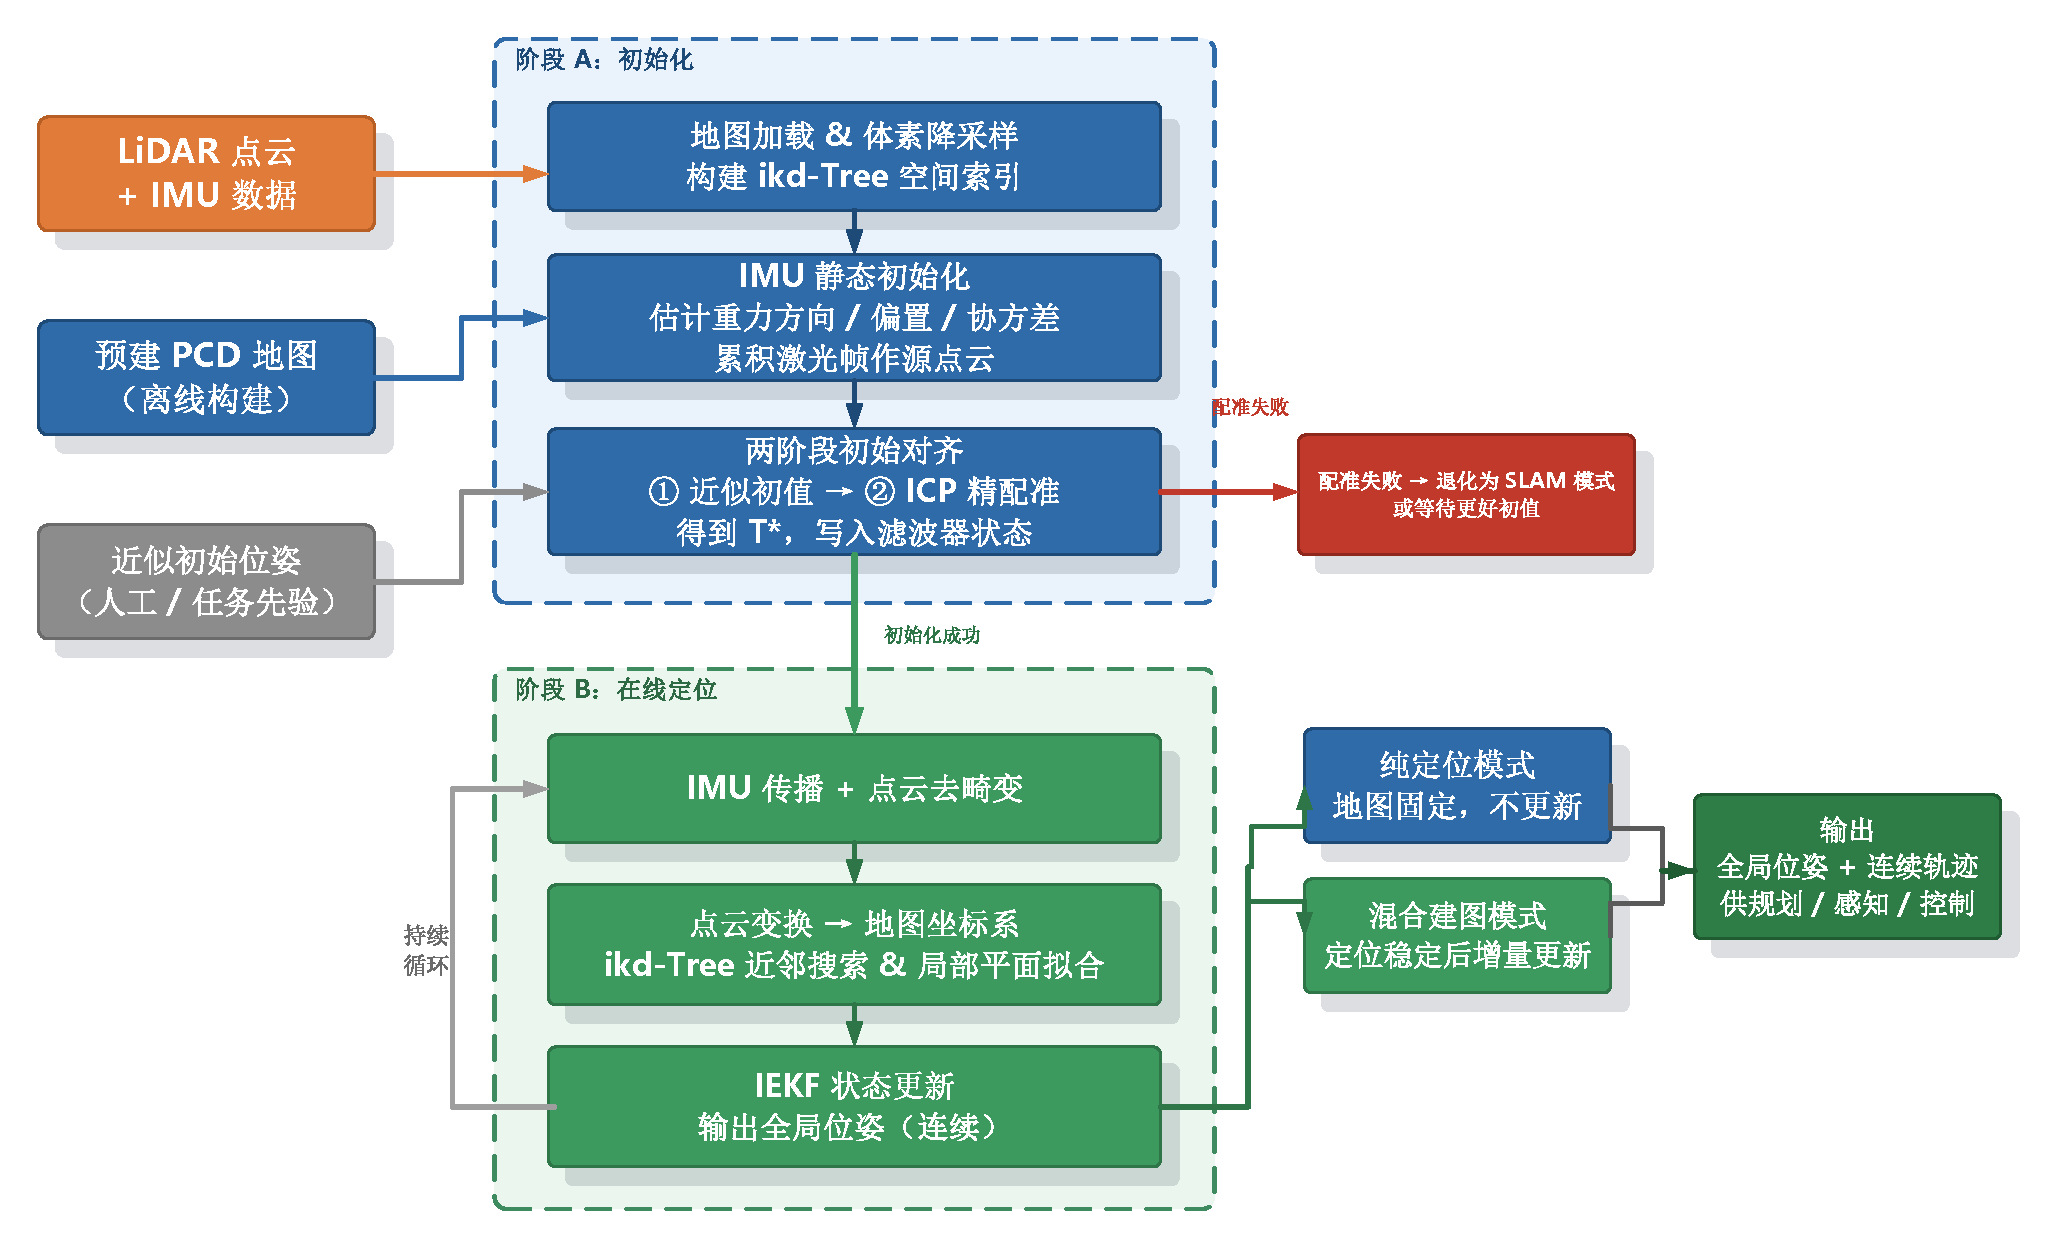
\includegraphics[width=0.92\linewidth]{pic/预建地图定位框架.pdf}
  \caption{基于预建地图的FAST-LIO2定位框架}
  \label{fig:map_localization}
\end{figure}

\subsection{预建地图定位框架}
预建地图定位系统的输入由三部分构成：一是连续到达的激光雷达点云和IMU测量，二是离线构建得到的全局点云地图，三是机器人在地图坐标系中的初始位姿近似。激光与惯性数据用于提供高频运动预测和局部几何观测，预建地图用于提供全局坐标基准，初始位姿近似则用于保证启动阶段点云配准能够收敛到正确邻域。

系统输出为地图坐标系下的机器人位姿、连续轨迹以及经位姿变换后的当前帧点云。对于上层路径规划和运动控制模块而言，该输出相当于全局定位反馈；对于感知和地图更新模块而言，该输出提供了将局部观测投影到统一坐标系的时变位姿。为了避免导航任务在定位尚未收敛前启动，系统在初始化完成前应保持任务锁定状态，待地图加载、IMU初始化和初始配准均满足条件后再向上层模块释放定位可用信号。

\subsection{预建地图加载与初始位姿对齐}
定位流程启动后，系统首先读取离线构建的PCD点云地图，并通过均匀采样或体素滤波降低冗余点密度。随后，以预建地图初始化增量式空间索引，使后续点云配准能够直接在全局地图中进行近邻搜索。完成该步骤后，地图不再只是里程计运行过程中逐步生成的局部几何集合，而是作为固定的全局几何先验参与后续每帧激光量测更新。

由于点云配准通常是局部优化问题，启动阶段需要较可靠的初始位姿。本文采用“近似初值 + ICP精配准”的两阶段初始化策略：首先由人工设定、停靠位置或上层先验给出机器人在预建地图中的粗略位姿；然后在IMU静态初始化完成后，累积若干帧激光点云形成局部源点云，并将其与预建地图进行ICP配准\textsuperscript{\cite{Besl1992ICP}}。ICP的目标可表示为
\begin{equation}
    \mathbf{T}^{*}
    =
    \arg\min_{\mathbf{T}\in SE(3)}
    \sum_{i}
    \left\|
    \mathbf{T}\mathbf{p}_{i}
    -
    \mathbf{q}_{\pi(i)}
    \right\|^{2},
    \label{eq:icp_init}
\end{equation}
其中$\mathbf{p}_{i}$为启动阶段累积的局部点云，$\mathbf{q}_{\pi(i)}$为预建地图中的对应点，$\mathbf{T}^{*}$为源点云到地图坐标系的最优刚体变换。ICP收敛后，得到的位姿修正被写入滤波器初始状态，使后续激光惯性状态估计直接在预建地图坐标系下展开。若初始配准无法收敛，则说明粗略位姿、当前观测或地图几何之间存在较大不一致，此时不应继续启动导航任务，以避免错误初值引起持续定位发散。

上述两阶段初始对齐过程如图\ref{fig:icp_align}所示。首先由近似初值将启动阶段累积的源点云$\mathbf{p}_{i}$粗略摆放到预建地图的正确邻域，此时源点云与地图之间仍存在明显的旋转和平移偏差（图\ref{fig:icp_align}(a)）；随后进入ICP迭代精配准，在每次迭代中先为源点建立到地图的最近邻对应$\mathbf{p}_{i}\leftrightarrow\mathbf{q}_{\pi(i)}$，再求解使式\eqref{eq:icp_init}最小的刚体变换并更新源点云位姿（图\ref{fig:icp_align}(b)），如此反复直至点对残差收敛至阈值$\varepsilon$；最终得到的最优变换$\mathbf{T}^{*}$将源点云精确对齐到地图坐标系（图\ref{fig:icp_align}(c)），并写入滤波器初始状态。其中点对残差是否收敛至阈值$\varepsilon$可作为初始化是否成功的判据，若残差无法收敛则放弃本次启动对齐。

\begin{figure}[htbp]
  \centering
  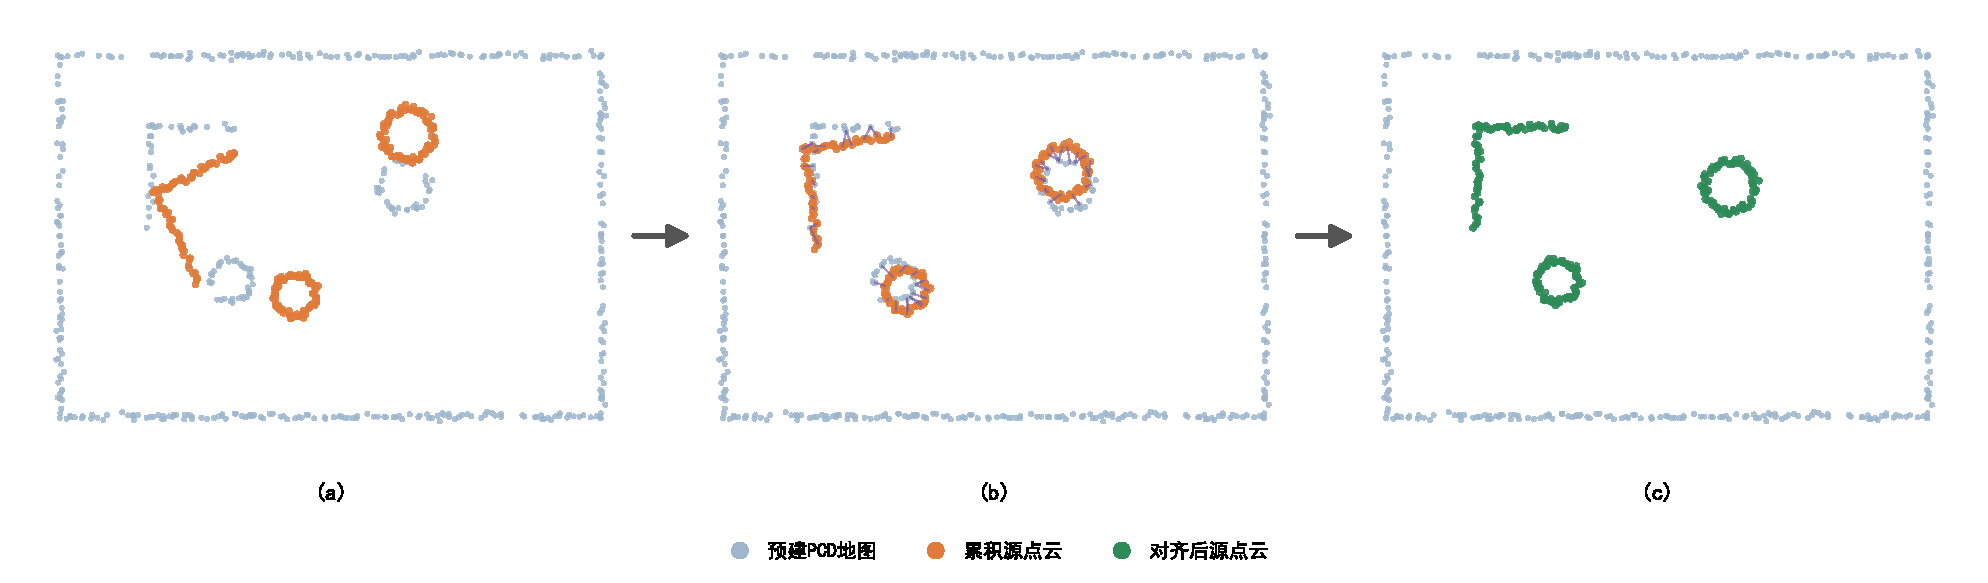
\includegraphics[width=\linewidth]{pic/两阶段ICP初始对齐.pdf}
  \caption{两阶段初始对齐过程示意}
  \label{fig:icp_align}
\end{figure}

\subsection{地图约束下的在线定位更新}
完成初始对齐后，系统进入逐帧定位阶段。每当激光点云与IMU数据完成时间同步，状态估计器首先根据IMU序列进行状态传播，并对当前帧点云进行运动畸变补偿；随后，将去畸变点云变换到地图坐标系，在预建地图中搜索近邻点并拟合局部平面，构造点到平面的残差；最后，通过迭代误差状态卡尔曼滤波更新机器人位姿、速度和IMU偏置。由于纯定位模式下地图保持固定，激光量测始终约束在同一全局地图坐标系内，输出位姿也自然具有全局一致性。

从算法结构看，该流程可抽象为以下步骤：

（1）加载预建点云地图，对地图点云进行降采样，并构建空间索引。

（2）利用启动阶段IMU数据估计重力方向、陀螺仪偏置和初始协方差，同时累积若干帧激光点云作为初始配准源点云。

（3）若预建地图有效，则以近似初值执行ICP配准，将得到的修正变换写入滤波器状态，并将定位状态标记为可用；若预建地图为空或点数不足，则退化为普通SLAM模式。

（4）在每一帧同步后的激光和IMU数据到来时，先进行IMU传播和点云去畸变，再将当前帧点云降采样并变换到地图坐标系。

（5）在地图索引中搜索近邻点并拟合局部平面，构造点到平面残差和量测雅可比，通过迭代卡尔曼滤波更新状态。若系统处于混合建图模式，则将满足条件的新观测增量并入地图。

\subsection{纯定位模式与混合建图模式}
根据地图是否随在线观测更新，本文方法可分为纯定位模式和混合建图模式。纯定位模式仅使用预建地图进行位姿估计，不将当前帧点云写入地图。这种模式适用于已经完成地图采集、巡检路线相对固定的场景，能够避免动态障碍物、临时设备或点云噪声污染全局地图。混合建图模式则在完成初始定位并稳定运行后允许地图增量更新，适用于预建地图不完整或机器人需要探索扩展区域的场景。此时新采集点云会在当前地图坐标系下并入地图，使扩展区域与原始地图保持同一坐标基准。

需要注意的是，本文所述重定位主要指系统启动或任务重启时基于近似初值的地图坐标恢复，而不是完全无先验的全局定位。由于ICP属于局部优化方法，初始位姿误差过大、环境几何重复、视场内有效结构过少或预建地图与当前环境差异过大时，配准可能收敛到错误局部最优。因此，在实际部署中应结合机器人停靠点、人工给定初值、二维码/定位桩、轮速里程计或上层任务先验提供合理初始位姿。同时，机器人应在地图加载和初始化期间保持静止，以保证IMU初始化和点云累积质量。

\section{本章算法特点与适用性分析}
相较于仅依赖轮式里程计或AMCL粒子滤波的二维定位方法，基于FAST\_LIO2的三维激光惯性定位具有以下优势。首先，三维点云能够直接利用墙面、设备支架、电缆沟边缘和立体障碍物等空间结构，在平面纹理不明显或二维激光可见特征不足时仍可提供较强约束。其次，IMU传播为高频状态估计和点云去畸变提供支撑，可提升机器人在转弯、加减速和短时遮挡条件下的定位连续性。再次，直接点到地图配准减少了特征提取阈值对不同雷达型号和扫描模式的依赖，有利于系统在不同传感器平台上的迁移。

该方法也存在一定局限。其一，FAST\_LIO2本质上仍是局部里程计框架，若脱离预建地图或回环后端，长距离运行会产生漂移；本文通过固定预建地图定位减轻该问题，但地图本身的质量会直接影响定位效果。其二，激光几何约束依赖足够丰富的空间结构，在长直走廊、开阔区域、单一大平面或近距离遮挡严重场景中可能出现退化。其三，该启动重定位策略依赖近似初值和ICP收敛性，不适合直接处理完全未知初始位置。针对上述问题，后续可进一步引入全局点云描述子、回环检测或多源传感器辅助定位，以提升全局重定位能力和长期运行稳定性。
\section{本章小结}
本章围绕移动机器人定位需求，研究了基于FAST\_LIO2的激光里程计定位算法。首先介绍了SLAM系统的基本架构和技术分类，分析了基于滤波器、基于图优化以及紧耦合激光惯性SLAM方法的特点。随后重点阐述FAST\_LIO2的核心原理，包括IMU状态传播、激光点云运动畸变补偿、直接点到地图残差、流形迭代卡尔曼滤波以及ikd-Tree增量地图维护机制。

在此基础上，本章说明了面向预建PCD地图的定位与启动重定位流程。系统通过加载预建地图构建空间索引，以近似初始位姿和ICP完成地图坐标系下的初始对齐，并在后续运行中利用FAST\_LIO2的点到平面量测更新持续输出全局位姿。通过区分纯定位模式和混合建图模式，所述方法能够在固定地图巡检和地图扩展两类任务之间切换，为后续路径规划、障碍物检测和导航控制模块提供稳定的位姿基础。
